\documentclass[11pt]{article}
\pdfoutput=1

\usepackage[margin=1.1in]{geometry}
\usepackage{amsmath,amssymb,amsthm}
\usepackage{booktabs}
\usepackage{microtype}
\usepackage{tikz}
\usetikzlibrary{arrows.meta,positioning}
\usepackage[hidelinks]{hyperref}

\theoremstyle{plain}
\newtheorem{theorem}{Theorem}
\newtheorem{lemma}[theorem]{Lemma}
\newtheorem{proposition}[theorem]{Proposition}
\newtheorem{corollary}[theorem]{Corollary}
\theoremstyle{definition}
\newtheorem{definition}[theorem]{Definition}
\theoremstyle{remark}
\newtheorem{remark}[theorem]{Remark}

\newcommand{\lift}{v(S) - v(\emptyset)}

\title{Principal Skill Analysis: Attributing Agent Performance\\to Individual Skills and Their Combinations}
\author{Joel Suro}
\date{Registered Report, Stage 1\\\today}

\begin{document}
\maketitle

\begin{abstract}
Coding agents are routinely extended with collections of written instructions, called skills or harnesses, that the agent can load on demand. Authors publish these collections and report that they help; organisations install them and pay for the tokens they consume. What no one can currently say is which parts of a collection produced the improvement, whether some parts do nothing at all, or whether one author's collection is better than another's, because the collections are evaluated whole and never against a shared baseline. In this work I propose Principal Skill Analysis (PSA), a measurement instrument that takes a skill collection as an input rather than studying one collection in particular, and that scores every skill against two outcomes given equal weight: tasks solved, and tasks solved per dollar.

The score assigned to a skill is its average contribution across every combination of other skills it might be loaded alongside, an allocation known as the Shapley value, which has the property that the individual scores add up to the improvement of the whole collection. A score per skill cannot say whether one skill is better paired with a second or a third, so PSA also measures every pair, and then compresses those pairwise measurements into a small number of independent areas of capability; keeping the best skill in each area gives a smaller collection that covers what the whole one covered.

Measuring every combination is impossible beyond a handful of skills, since a catalogue of $N$ skills has $2^N$ possible subsets: at $N = 39$, over five hundred billion. The exponential barrier turns out to be a property of enumeration rather than of the problem. Rewriting the value function in the basis of its dividends, the part of each combination's worth that no smaller combination accounts for, and assuming those vanish above interaction order $t$, leaves the attributions determined by $O(N^t)$ numbers rather than $2^N$: $781$ instead of $5.5 \times 10^{11}$ for pairs at $N = 39$. Within the assumption the result is exact rather than approximate, and I prove how many runs recovering it takes, that the required design resolution is $2t+1$, and how the assumption itself is tested against held-out configurations rather than trusted. A cheaper screening route is retained as a fallback for smaller budgets, with a proof that it does not discard the skills that work only in company. Noise is handled by comparing configurations on the same task rather than by buying more runs, and two controls make the measurements attributable at all: a skill matched in length but empty of instruction, whose score must come out indistinguishable from zero, and a record of whether the agent actually invoked each skill rather than merely having it available.

Existing work has applied this style of attribution to four or five hand-chosen agent modules. The contribution here is doing it at the scale of a real published catalogue, on collections practitioners actually install, and distinguishing a skill that was offered from a skill that was used. I predict that a small minority of skills accounts for most of the measurable gain, that many contribute nothing distinguishable from zero, that the gap between offered and used is large enough to reorder the ranking, and that which skills are loaded matters more for performance, and for what performance costs, than how large the collection is or who wrote it.
\end{abstract}

\section{Introduction}

Coding agents built on large language models are now routinely extended with collections of written instructions that the model can load on demand. These collections go by different names across ecosystems, and their authors describe them in the vocabulary of software engineering practice: test-first development, systematic debugging, verification before completion, planning before implementation. A collection is published, adopted, and defended, and the defence takes the form of an assertion that the collection improves outcomes.

The assertion is rarely accompanied by a measurement, and when it is, the measurement is aggregate. A collection is evaluated whole. This leaves three questions unanswered, and they are the questions a practitioner actually has.

The first is \emph{attribution}. If a collection of twenty skills improves a benchmark by some margin, which of the twenty produced the margin? Aggregate evaluation cannot say. It is entirely consistent with the observed data that two skills produced the entire effect and eighteen produced none, and equally consistent that all twenty contributed evenly. These two worlds imply opposite recommendations to a practitioner deciding what to load into a limited context window.

The second is \emph{combination}. The standard remedy for attribution is the ablation: remove one component, observe the change. This procedure conflates two different things. A skill that contributes nothing and a skill that contributes only in the presence of another both appear null under leave-one-out ablation, because removing either one from the full collection leaves the rest to compensate. The distinction matters, because the second kind of skill is not removable and the first kind is.

The third is \emph{comparability}. Two collections published by two authors cannot be compared because they were never measured against the same baseline, the same model, or the same seeds. Each author reports a number computed under their own conditions, and the numbers do not meet.

These questions are not only academic. An organisation running agents at scale pays for every token a loaded skill contributes to a prompt and for every turn it induces, and it pays whether or not the skill was ever invoked. Skill collections are adopted the way dependencies are adopted, by reputation and by star count, but unlike dependencies their cost is metered continuously and their benefit has never been measured. The practical form of the attribution question is therefore a budgeting question: given a fixed context budget, which skills belong in it, and how much of what is currently being paid for is buying nothing.

I address all three by treating the collection as an input to a measurement instrument rather than as the subject of a bespoke study. The instrument accepts a collection identified by repository and commit, evaluates it against a fixed baseline agent on a fixed benchmark, and returns a per-skill attribution with confidence intervals, the interaction structure among those skills, a decomposition into orthogonal areas of capability, and, given more than one collection, a comparison on a common footing.

This document is a pre-registration. The design, the hypotheses and the analysis plan are fixed here, before data collection, because the space of configurations is large enough that a determined analyst can always find a configuration producing an attractive result. A study of this shape that is not pre-registered is not defensible, and I would not believe one.

\section{Terms}
\label{sec:terms}

Four words are used throughout in a specific sense, and everything else technical is defined where it first appears.

A \emph{skill} is one written instruction file that an agent can load, of the kind published in the collections this work measures. A \emph{catalogue} is a set of such files, identified by the repository and revision it came from. A \emph{configuration} is the subset of a catalogue made available to the agent for one attempt at one task; it may be empty, a single skill, or all of them. A \emph{run} is one such attempt: one agent, one task, one configuration. Every later section uses these four words as defined here.

The quantity every measurement here refers back to is the \emph{lift}: how much better the agent does with the whole catalogue loaded than with none of it.

\section{Related Work}

\paragraph{Benchmarks for coding agents.} SWE-bench \cite{swebench} established the practice of evaluating agents on real repository issues with automated verification through the repository's own test suite, and SWE-bench Verified \cite{verified} produced a human-validated subset in which the tests are known to discriminate correct from incorrect patches. The binary pass-or-fail outcome these benchmarks provide is what makes the present design feasible: without an automatic and trustworthy verdict, the number of runs required could not be graded. Agent harnesses evaluated on them, such as SWE-agent \cite{sweagent}, are reported as complete systems, which is the aggregate reporting this work seeks to decompose.

\paragraph{Reported gains that do not survive controlled comparison.} The suspicion motivating this work is not novel, and it is not cynicism. In field after field, a body of claimed architectural progress has been re-examined under a controlled budget and found to be largely an artefact of unequal tuning. Lucic et al. \cite{lucic} compared generative adversarial networks under matched computational budgets and found that most models reached similar scores, with the reported differences attributable to tuning and random restarts rather than to the algorithmic changes credited with them. Melis et al. \cite{melis} re-evaluated recurrent language-model architectures under large-scale black-box hyperparameter search and found that a properly regularised standard LSTM outperformed the newer models said to have superseded it. Ferrari Dacrema et al. \cite{dacrema} reproduced recent neural recommendation methods and found that most were outperformed by simple, long-established baselines that had been tuned with comparable care. Musgrave et al. \cite{musgrave} found the same pattern in deep metric learning, where a decade of claimed improvement was marginal once the experimental protocol was equalised.

The common structure of these results is instructive for the present study. In each case the reported improvement was real as measured and misattributed as explained: the gain existed, but it belonged to a factor the authors were not varying deliberately. Skill collections are in exactly the position those architectures were in, with the additional difficulty that their components are never varied separately at all. What corrected the record in each case was not argument but a controlled comparison at equal budget, which is what this instrument is built to run.

\paragraph{Statistical practice in benchmark comparison.} Bouthillier et al. \cite{bouthillier} model the benchmarking process itself and show that concluding one method beats another requires accounting for several sources of variance simultaneously, of which the choice of data sample is frequently dominant. Agarwal et al. \cite{agarwal} make a closely related argument for reinforcement learning and recommend stratified bootstrap confidence intervals and performance profiles across tasks and runs in place of point comparisons. The task-paired design and the task-level bootstrap of Section~\ref{sec:power} follow their recommendations, applied to a setting where the unit of blocking is the benchmark task.

\paragraph{Sensitivity to prompt surface and to context.} The length-matched placebo of Section~\ref{sec:controls} is required by known results rather than adopted as good hygiene. Sclar et al. \cite{sclar} show that semantically equivalent reformattings of a prompt move accuracy by as much as tens of points on open models, and that the sensitivity persists as model size and shot count increase. Liu et al. \cite{lostmiddle} show that where information sits inside a long context materially changes whether a model uses it. A skill is delivered as text placed into a context window, so both effects operate on it directly: loading any skill changes prompt surface and context occupancy at once. Without a control matched on length, an attribution cannot be separated from those two mechanisms.

\paragraph{Attribution by Shapley value.} The Shapley value \cite{shapley} was introduced to distribute the payoff of a cooperative game among its players. Its adoption in machine learning has been broad: SHAP \cite{shap} applies it to feature attribution, and Data Shapley \cite{datashapley} to valuing training examples. Both face the same computational obstacle that appears here---the number of coalitions grows exponentially---and both answer it with sampling. I take a different route, in Section~\ref{sec:design}, because the effect sizes expected here are small enough that a sampling estimator's variance would dominate the quantity estimated. Covert et al. \cite{sage} take the step closest to the present work by applying the construction not to individual predictions but to a global measure of predictive power, which is structurally what $v$ is here. The permutation-sampling estimator used for the validation pass of Section~\ref{sec:validation} is that of Castro et al. \cite{castro}. The generalisation to interactions among players is due to Grabisch and Roubens \cite{grabisch}.

\paragraph{Attribution applied to agent components.} The construction this work uses has already been applied to agent systems, and the closest results should be stated plainly rather than left for a reader to discover. Yang et al. \cite{shapleyflow} score the modules of an agentic workflow, such as planning and reflection, by their average contribution across configurations, across seven task families. Liu \cite{mliu} runs every one of the $2^5 = 32$ combinations of five scaffolding components on two benchmarks, computes the same scores without approximation, reports interaction measurements including one three-way term, and finds that switching everything on is worse than switching on a subset: a single-tool agent beat the fully equipped one by $32\%$ on one benchmark. Li et al. \cite{skillsv} score the parts inside a single skill, using a padding scheme that holds prompt length constant so that content is separated from the cost of the context it occupies. Liu et al. \cite{skillshapley} attribute value to individual steps within a skill.

Three things about that body of work bear on what remains to be done. Every one of these studies operates on four or five modules chosen by hand, or on the parts of one skill. At that size every combination can simply be run, so the problem of measuring a catalogue too large to enumerate does not arise, and neither does the question of how to reach it without discarding the components that work only in company. None of them records whether a component was actually used, because in their designs a component is wired in: if the memory module is enabled, it runs. A skill offered to an agent by a one-line descriptor may never be invoked at all, which makes the distinction between offered and used unavoidable here and absent there. And none of them takes a published catalogue as an input, so none can compare one author's collection against another's on a shared baseline, which is the comparison practitioners actually face.

\paragraph{Design of experiments.} Identifying which of many factors matter using far fewer runs than the full factorial is a solved problem. Plackett--Burman designs \cite{plackett} estimate $N$ main effects in a number of runs proportional to $N$, and the foldover construction that raises such a design from Resolution~III to Resolution~IV is standard \cite{bhh}.

\paragraph{Pre-registration.} The Registered Report format \cite{chambers} was introduced in response to the structural problem this study faces: large analytic degrees of freedom combined with an incentive to report positive findings.

\paragraph{Prior work by the author.} The concern motivating this study---that probabilistic systems are routinely reported as more reliable than their verification supports---also motivated earlier work on introducing deterministic evaluation into retrieval-augmented generation \cite{suro}. The present work applies the same instinct one level up, to the evaluation of agent scaffolding itself.

\section{Problem Formulation}

\subsection{The chain of reasoning}

Each choice below is forced by the failure of the choice before it.

The quantity of interest is the \emph{lift}, $\lift$: how much better an agent performs with a collection loaded than without. Every author reports some version of this number; the question is how it is produced. The obvious attribution---the ablation---fails, for the reason given in Section~1. Fixing it requires evaluating a skill across many contexts rather than one, so that its worth is the average of its marginal contributions over the coalitions it might join. That is a definition and not yet a method, since many averages satisfy it. Requiring the average to be \emph{fair}, in a sense made precise in Section~\ref{sec:axioms}, fixes it uniquely. But the resulting estimator requires the value function on all $2^N$ subsets, which is unavailable at realistic catalogue sizes, so coverage rather than exactness must give: a balanced screen costing $O(N)$ runs identifies the skills worth pursuing and the exact computation runs over those alone. That screen must not discard the combination-only skills the study exists to find, which is guaranteed by Lemma~\ref{lem:balance}. The exact stage then measures every interaction order at once, but a per-skill number discards them, so the interaction index is reported alongside; and a per-pair number does not scale into a decision, so the interaction matrix is decomposed into orthogonal areas by Lemma~\ref{lem:block}.

\subsection{What is executed and what is computed}

A \emph{run} is one agent attempt at one benchmark task with one \emph{configuration} loaded, where a configuration is any subset of the catalogue---empty, a single skill, twenty skills, or all of them. Nothing in this design is executed pairwise. Pairs, triples and areas are computed \emph{from} those runs during analysis. A screening run at a catalogue of $39$ skills loads roughly twenty skills at once, by construction of the balanced design.

\subsection{Notation}

Let $S = \{s_1,\dots,s_N\}$ be the catalogue under test and let a configuration $C \subseteq S$ be the subset available to the agent during a run. Let $T$ be the set of benchmark tasks and $Y(t,C,r)$ the outcome of run $r$ on task $t$ under configuration $C$. Define the value function
\[
v(C) = \mathbb{E}_{t \in T,\, r}\big[Y(t,C,r)\big],
\]
so that $v(\emptyset)$ is the bare agent and $v(S)$ the agent with the whole catalogue available.

\section{Building the Attribution from the Ground Up}
\label{sec:axioms}

This section constructs the estimator rather than selecting it. Nothing below is invoked on authority: the formula is derived, the properties that matter are proved, and only the uniqueness result at the end is taken from the literature, with the reason it is not reproved stated plainly.

\subsection{Marginal contribution along an ordering}

Start from the only thing that can be measured directly. Suppose the skills are introduced one at a time in some order, each added to those already present. Then each skill has an unambiguous contribution: what the agent gained at the moment it was added.

\begin{definition}\label{def:order}
Let $\pi$ be a permutation of $S$, and let $P_i^\pi = \{ j \in S : \pi(j) < \pi(i)\}$ be the set of skills preceding $i$ in $\pi$. The marginal contribution of $i$ along $\pi$ is
\[
\Delta_i^\pi \;=\; v\big(P_i^\pi \cup \{i\}\big) \;-\; v\big(P_i^\pi\big).
\]
\end{definition}

This quantity has no ambiguity and no modelling assumption in it. Both terms are configurations that can be run, and their difference is what adding the skill bought in that context.

\begin{proposition}\label{prop:telescope}
For every ordering $\pi$, $\;\sum_{i \in S} \Delta_i^\pi = \lift$.
\end{proposition}

\begin{proof}
Write the skills in the order given by $\pi$ as $i_1, i_2, \dots, i_N$, and let $C_m = \{i_1,\dots,i_m\}$ with $C_0 = \emptyset$. By Definition~\ref{def:order}, $\Delta_{i_m}^\pi = v(C_m) - v(C_{m-1})$. Summing over $m = 1,\dots,N$,
\[
\sum_{m=1}^{N} \big(v(C_m) - v(C_{m-1})\big) \;=\; v(C_N) - v(C_0) \;=\; \lift,
\]
every intermediate term cancelling against its neighbour.
\end{proof}

Proposition~\ref{prop:telescope} is the reason this starting point is the right one. Along any single ordering the contributions already add up to exactly the lift, with nothing left over and nothing double counted. The difficulty is that $\Delta_i^\pi$ depends on $\pi$: a skill introduced first is credited with work that a skill introduced last would have been credited with instead. A skill that only functions alongside another receives everything when it arrives second and nothing when it arrives first.

\subsection{Averaging over orderings, and where the weights come from}

Since no ordering is privileged, treat them all alike.

\begin{definition}\label{def:shapley}
$\displaystyle \varphi_i \;=\; \frac{1}{N!}\sum_{\pi} \Delta_i^\pi$, the average over all $N!$ orderings.
\end{definition}

\begin{proposition}\label{prop:weights}
$\displaystyle \varphi_i \;=\; \sum_{C \subseteq S \setminus \{i\}} \frac{|C|!\,(N - |C| - 1)!}{N!}\Big[v(C \cup \{i\}) - v(C)\Big].$
\end{proposition}

\begin{proof}
Group the $N!$ orderings by the predecessor set they induce for $i$. Fix $C \subseteq S \setminus \{i\}$ with $|C| = c$. An ordering satisfies $P_i^\pi = C$ when, and only when, the $c$ elements of $C$ occupy the first $c$ positions in some order, $i$ occupies position $c+1$, and the remaining $N - c - 1$ skills follow in some order. There are $c!$ arrangements of the first group and $(N-c-1)!$ of the last, so exactly $c!\,(N-c-1)!$ orderings induce that predecessor set. Every ordering induces exactly one such set, so the groups partition the $N!$ orderings. Within a group, $\Delta_i^\pi = v(C \cup \{i\}) - v(C)$ is constant. Substituting into Definition~\ref{def:shapley} gives the claim.
\end{proof}

The combinatorial weight is therefore not a convention. It is the fraction of orderings in which a skill happens to arrive with exactly that set of predecessors, which is why coalitions of extreme size receive the larger weights: there are few ways to arrive first or last, and many ways to arrive in the middle.

\subsection{What this construction already guarantees}

Three properties follow immediately, and each answers a question a practitioner has.

\begin{proposition}[Additivity of the decomposition]\label{prop:eff}
$\sum_{i \in S} \varphi_i = \lift$.
\end{proposition}

\begin{proof}
Averaging Proposition~\ref{prop:telescope} over $\pi$ and exchanging the two finite sums.
\end{proof}

Proposition~\ref{prop:eff} is what licenses the central claim of any attribution plot. The individual numbers add to what the whole collection delivered, so a statement such as ``these three skills account for eighty per cent of the benefit'' has a referent and needs no normalisation. Without this property such a statement is a ranking dressed as a decomposition.

\begin{proposition}[An inert skill scores exactly zero]\label{prop:null}
If $v(C \cup \{i\}) = v(C)$ for every $C \subseteq S\setminus\{i\}$, then $\varphi_i = 0$.
\end{proposition}

\begin{proof}
Every $\Delta_i^\pi$ in Definition~\ref{def:shapley} vanishes term by term.
\end{proof}

This is the property a practitioner needs in order to justify not loading something. An estimator that assigns small positive noise to an inert skill supplies no ground for dropping anything, and what to drop is the central practical question here.

\begin{proposition}[Interchangeable skills score alike]\label{prop:sym}
If $v(C \cup \{i\}) = v(C \cup \{j\})$ for every $C \subseteq S \setminus \{i,j\}$, then $\varphi_i = \varphi_j$.
\end{proposition}

\begin{proof}
Pair each ordering $\pi$ with the ordering $\pi'$ obtained by swapping the positions of $i$ and $j$. Applying the swap twice returns the original ordering, so the pairing matches every ordering with one other and covers all of them, and $\Delta_i^\pi = \Delta_j^{\pi'}$ by hypothesis, so the two averages coincide.
\end{proof}

Symmetry matters here beyond fairness: one hypothesis of this work concerns authorship and provenance, so an estimator with any sensitivity to a skill's name or position would beg the question it is meant to test.

\begin{proposition}[Linearity]\label{prop:lin}
For value functions $v, w$ on $S$ and scalars $a,b$, $\;\varphi_i(av + bw) = a\varphi_i(v) + b\varphi_i(w)$.
\end{proposition}

\begin{proof}
$\Delta_i^\pi$ is a difference of two evaluations of the value function, hence linear in it, and Definition~\ref{def:shapley} is a finite average of such differences.
\end{proof}

Proposition~\ref{prop:lin} is not decoration. It is the machinery that makes the study affordable. Because $\varphi$ is linear in $v$, computing the attribution separately for each task and then averaging over tasks gives the same answer as attributing the task-averaged value function. That identity is what permits the task-paired analysis of Section~\ref{sec:power}, which removes the dominant source of variance. The explicit weights of Proposition~\ref{prop:weights} are what the implementation computes. Had the construction not been linear, the blocking would not have been available and the required sample size would have been unreachable.

\subsection{Why stop here}

The construction above is one particular way of averaging. It is fair to ask whether some other average would serve better. The answer is that no other one satisfies the four properties just proved.

\begin{theorem}[Shapley, 1953]\label{thm:shapley}
$\varphi$ as given in Definition~\ref{def:shapley} is the unique map from value functions to attributions satisfying Propositions~\ref{prop:eff}, \ref{prop:null}, \ref{prop:sym} and \ref{prop:lin}.
\end{theorem}

Linearity is the property most often disputed in machine-learning applications of this construction, so it is worth recording that the result does not depend on it. Young \cite{young} shows that linearity can be dropped entirely and replaced by monotonicity, the requirement that a skill whose contribution to every coalition rises should not be credited with less, and that the same estimator is again the unique one satisfying the remaining properties. A reader who rejects linearity therefore does not obtain a different estimator; they obtain the same one from a different and arguably more intuitive premise. That the construction is reachable from two independent directions is stronger evidence for it than either axiomatisation alone.

Theorem~\ref{thm:shapley} is the one result in the section taken from the literature rather than proved, and the reason is worth stating: the uniqueness argument is a linear-algebraic decomposition of the space of value functions into unanimity games, and reproducing it here would add length without adding assurance, since it is standard and has been checked for seventy years. See \cite{shapley}. What the theorem contributes to the present argument is that the four properties are not a wish list from which a convenient estimator may be picked. By Theorem~\ref{thm:shapley} they admit exactly one estimator, so any disagreement about the estimator is a disagreement about the properties, which is where such an argument belongs.

\subsection{Why the usual objection to Shapley attribution does not apply here}

\begin{remark}\label{rem:interventional}
A known criticism of Shapley-based attribution in machine learning \cite{kumar} is that the value of a coalition is not measured but simulated. Absent features are marginalised out of a model trained on all of them, so $v(C)$ is evaluated at inputs the model never saw, and the resulting attributions depend on the imputation scheme as much as on the system.

That criticism does not reach this design. Every coalition here is physically realised: the agent is executed with the skills of $C$ available and no others, which an automated check verifies for every run by confirming that the workspace contains the files of $C$ and no others. No value is imputed. Each $v(C)$ is an average of outcomes that were observed. The value function is what statisticians call \emph{interventional}: it reports what happened when the world was changed, rather than what a model predicts would happen if it had been, and the attributions are attributions of an intervention rather than of a model's response to an input unlike anything it was trained on.
\end{remark}

\section{Design}
\label{sec:design}

The full factorial is unavailable: the subset space contains $2^N$ configurations, where the $2$ is the presence or absence of each skill---two states per skill---and not, as the notation invites one to read, a pairing. At $N = 39$ this is over $5.5 \times 10^{11}$ configurations. The design proceeds in two stages with a validation pass, illustrated in Figure~\ref{fig:funnel}.

\begin{figure}[t]
\centering
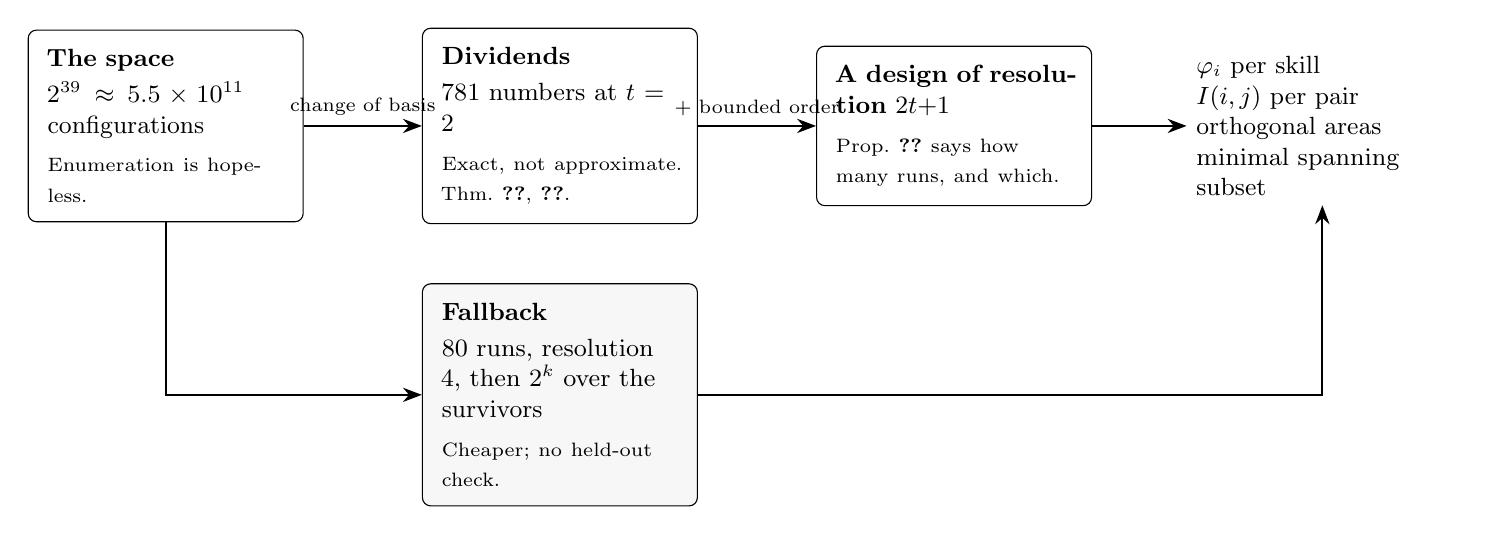
\begin{tikzpicture}[
  box/.style={draw, rounded corners=3pt, minimum height=2.0cm, text width=3.0cm, align=left, inner sep=7pt, font=\small},
  arr/.style={-{Stealth[length=2.4mm]}, thick},
  lbl/.style={font=\scriptsize, midway, above}
]
\node[box] (a) {\textbf{The space}\\[2pt] $2^{39} \approx 5.5\times10^{11}$ configurations\\[3pt] \scriptsize Enumeration is hopeless.};
\node[box, right=1.5cm of a] (b) {\textbf{Dividends}\\[2pt] $781$ numbers at $t=2$\\[3pt] \scriptsize Exact, not approximate. Thm.~\ref{thm:mobius}, \ref{thm:shapmobius}.};
\node[box, right=1.5cm of b] (c) {\textbf{A design of resolution $2t{+}1$}\\[3pt] \scriptsize Prop.~\ref{prop:resolution} says how many runs, and which.};
\node[right=1.2cm of c, text width=3.2cm, align=left, font=\small] (d) {$\varphi_i$ per skill\\ $I(i,j)$ per pair\\ orthogonal areas\\ minimal spanning subset};
\node[box, below=0.75cm of b, fill=black!3] (f) {\textbf{Fallback}\\[2pt] $80$ runs, resolution $4$, then $2^k$ over the survivors\\[3pt] \scriptsize Cheaper; no held-out check.};
\draw[arr] (a) -- node[lbl]{\scriptsize change of basis} (b);
\draw[arr] (b) -- node[lbl]{\scriptsize $+$ bounded order} (c);
\draw[arr] (c) -- (d);
\draw[arr] (a.south) |- (f.west);
\draw[arr] (f.east) -| (d.south);
\end{tikzpicture}
\caption{The primary route rewrites the value function in a basis where bounded interaction order makes the problem polynomial, and tests that assumption against held-out configurations. The screening route below is retained for budgets that will not stretch to $p$ configurations, and has no comparable check.}
\label{fig:funnel}
\end{figure}

\subsection{A change of basis that makes the problem polynomial}
\label{sec:mobius}

Enumerating every configuration is unnecessary, and the reason is a change of basis rather than an approximation.

\begin{definition}\label{def:mobius}
For a value function $v$ on $2^S$, define for each $T \subseteq S$
\[
a(T) \;=\; \sum_{L \subseteq T} (-1)^{|T| - |L|}\, v(L).
\]
The numbers $a(T)$ are the \emph{dividends} of the game, after Harsanyi.
\end{definition}

\begin{theorem}[Representation]\label{thm:mobius}
For every $C \subseteq S$, $\;v(C) = \sum_{T \subseteq C} a(T)$, and the numbers $a(T)$ are the only ones with this property.
\end{theorem}

\begin{proof}
Substitute Definition~\ref{def:mobius} and exchange the order of summation:
\[
\sum_{T \subseteq C} a(T) \;=\; \sum_{T \subseteq C}\ \sum_{L \subseteq T} (-1)^{|T|-|L|} v(L) \;=\; \sum_{L \subseteq C} v(L) \sum_{T \,:\, L \subseteq T \subseteq C} (-1)^{|T|-|L|}.
\]
Fix $L$ and put $m = |C \setminus L|$. The sets $T$ with $L \subseteq T \subseteq C$ are obtained by adding to $L$ any of the $m$ remaining elements, so grouping them by how many were added gives
\[
\sum_{T \,:\, L \subseteq T \subseteq C} (-1)^{|T|-|L|} \;=\; \sum_{j=0}^{m} \binom{m}{j} (-1)^{j} \;=\; (1-1)^{m},
\]
by the binomial theorem. That is $0$ whenever $m > 0$ and $1$ when $m = 0$, which happens only for $L = C$. Every term therefore vanishes except $v(C)$, proving the identity.

For uniqueness, note that both directions are linear maps on the $2^{|S|}$-dimensional space of functions on subsets, and the display above shows that the map $a \mapsto v$ inverts the map $v \mapsto a$. A linear map with a two-sided inverse is a bijection, so no second family of coefficients can represent the same $v$.
\end{proof}

The dividends have a direct reading. Since $a(\{i\}) = v(\{i\}) - v(\emptyset)$, a first-order dividend is what a skill is worth alone. Since $a(\{i,j\}) = v(\{i,j\}) - v(\{i\}) - v(\{j\}) + v(\emptyset)$, a second-order dividend is what the pair is worth beyond the two of them separately. Higher orders continue the pattern: $a(T)$ is the part of the value of $T$ that no proper subset of $T$ accounts for.

\begin{theorem}[The attribution in terms of dividends]\label{thm:shapmobius}
$\displaystyle \varphi_i \;=\; \sum_{T \,\ni\, i} \frac{a(T)}{|T|}.$
\end{theorem}

\begin{proof}
For $T \neq \emptyset$ let $u_T$ be the value function that is $1$ on configurations containing all of $T$ and $0$ otherwise. Theorem~\ref{thm:mobius} says $v = a(\emptyset) + \sum_{T \neq \emptyset} a(T)\, u_T$, and adding a constant to $v$ changes no marginal contribution, so by linearity (Proposition~\ref{prop:lin}) it suffices to compute $\varphi_i(u_T)$ for a single $T$.

Fix $T$ and an ordering $\pi$. By Definition~\ref{def:order}, $\Delta_i^{\pi} = u_T(P_i^\pi \cup \{i\}) - u_T(P_i^\pi)$, which is $1$ when the first of the two configurations contains $T$ and the second does not, and $0$ otherwise. That happens when $i \in T$ and every other member of $T$ precedes $i$: in other words, when $i$ is the last member of $T$ to appear. If $i \notin T$, adding $i$ can never complete $T$, so every $\Delta_i^\pi$ is $0$ and $\varphi_i(u_T) = 0$.

Suppose $i \in T$. Averaging over orderings, $\varphi_i(u_T)$ is the fraction of orderings in which $i$ is the last of the $|T|$ members of $T$. The restriction of a uniformly random ordering of $S$ to the members of $T$ is a uniformly random ordering of $T$, and each of its $|T|$ members is equally likely to be last, so that fraction is $1/|T|$.

Summing over $T$ with the coefficients $a(T)$ gives the claim.
\end{proof}

Theorem~\ref{thm:shapmobius} says the attribution splits each dividend equally among the skills that earned it. It also re-derives additivity independently of Proposition~\ref{prop:eff}: summing over $i$ gives $\sum_i \varphi_i = \sum_{T \neq \emptyset} a(T) \sum_{i \in T} 1/|T| = \sum_{T \neq \emptyset} a(T)$, and by Theorem~\ref{thm:mobius} that is $v(S) - a(\emptyset) = \lift$. Two independent routes to the same identity is a useful check on both.

\subsection{What bounded interaction order buys}

\begin{corollary}[Complexity]\label{cor:complexity}
Suppose $a(T) = 0$ for every $T$ with $|T| > t$. Then $v$ and all the attributions $\varphi_i$ are determined by
\[
p \;=\; \sum_{j=0}^{t} \binom{N}{j}
\]
numbers, which grows as $O(N^t)$.
\end{corollary}

\begin{proof}
Immediate from Theorems~\ref{thm:mobius} and \ref{thm:shapmobius}: both expressions are sums over subsets, and every term with $|T| > t$ is zero, leaving only subsets of size at most $t$, of which there are $p$.
\end{proof}

Nothing in this change of basis reintroduces the difficulty Remark~\ref{rem:interventional} rules out: every $v(L)$ entering Definition~\ref{def:mobius} is an average of runs that were executed, so the dividends are computed from measurements throughout.

The saving is not marginal. At $N = 39$ and $t = 2$ the catalogue has $2^{39} \approx 5.5 \times 10^{11}$ configurations but only $1 + 39 + 741 = 781$ dividends, and $780$ of them enter the attributions. The problem stops being exponential and becomes polynomial.

What has been paid for this is an assumption, not an approximation: within the assumption the attributions are exact. Everything therefore depends on whether the assumption holds, which is the subject of Section~\ref{sec:faithful}. It is not idle: the design-of-experiments literature calls the corresponding regularity the sparsity-of-effects principle \cite{bhh}, and it has been observed directly in language models, where interactions among input features are both sparse and hierarchical, with high-order terms appearing alongside their lower-order subsets \cite{spex,proxyspex}.

\subsection{How many runs bounded order requires}

Corollary~\ref{cor:complexity} counts unknowns. Recovering them requires a design that separates them, which is where the language of resolution earns its place.

Encode a configuration (Section~\ref{sec:terms}) as $x \in \{-1,+1\}^N$ with $x_j = +1$ when skill $j$ is loaded, and for $A \subseteq S$ write $x_A = \prod_{j \in A} x_j$, with $x_\emptyset = 1$. Every value function on configurations can be written as $\sum_{A} \theta_A\, x_A$, and the assumption of Corollary~\ref{cor:complexity} is that $\theta_A = 0$ for $|A| > t$. This is the same statement in a different coding; the two sets of coefficients are related by an invertible change of variables.

Estimate $\theta_A$ by the contrast $\hat\theta_A = \frac{1}{n}\sum_{r} x_{rA}\, y_r$. Two effect terms are indistinguishable when their columns coincide, and since every entry is $\pm 1$ and therefore squares to one,
\[
x_A x_B \;=\; x_{A \,\triangle\, B},
\]
where $A \triangle B$ is the set of skills in one of $A$ and $B$ but not both. So the columns of $A$ and $B$ coincide precisely when $x_{A \triangle B}$ is the all-ones column. Call a non-empty set $W$ with $x_W$ all-ones a \emph{defining word} of the design, and call the \emph{resolution} $R$ the size of its shortest defining word. This is where the numeral in ``Resolution IV'' comes from: it counts skills in the shortest confusion the design admits.

\begin{proposition}[Required resolution]\label{prop:resolution}
All effects of order at most $t$ are separately estimable if and only if the design has resolution $R \ge 2t+1$.
\end{proposition}

\begin{proof}
Two effects $A \neq B$ with $|A|,|B| \le t$ are confounded when $A \triangle B$ is a defining word. Since $A \triangle B$ is non-empty and $|A \triangle B| \le |A| + |B| \le 2t$, a design with a defining word of length at most $2t$ admits such a pair, and conversely if the shortest defining word has length at least $2t+1$ then no $A \triangle B$ of size at most $2t$ can be one, so no two effects of order at most $t$ are confounded.
\end{proof}

Proposition~\ref{prop:resolution} makes the design choice a consequence rather than a preference. Measuring every pair, $t = 2$, requires resolution $5$. Measuring only which skills matter, $t = 1$, requires resolution $3$; separating those main effects from pairs, so that a skill working only in company is not lost, requires resolution $4$, which is the case discussed in Section~\ref{sec:screen}. A design must also have at least $p$ runs, since $p$ unknowns cannot be recovered from fewer equations.

\subsection{Testing the assumption instead of trusting it}
\label{sec:faithful}

Bounded order is the one substantive assumption in this design, so it is measured rather than asserted.

Configurations are split before fitting into an estimation set and a held-out set, the split fixed by seed in the pre-registration. The order-$t$ coefficients are fitted on the estimation set alone, and used to predict the value of each held-out configuration, which the fit never saw. Two numbers are then compared: the mean squared prediction error on the held-out configurations, and the variance of repeated runs of the same configuration, which is the error floor no model can go below.

If the assumption holds, held-out error is at the level of that floor: the order-$t$ model is describing everything except noise. If held-out error stands clearly above the floor, interactions above order $t$ carry real signal, the assumption is wrong, and the reported attributions are incomplete. The threshold at which that verdict is declared is fixed in the pre-registration, and a failed test is reported as a failed test. The quantity is what \cite{spex} calls faithfulness, used there for the same purpose.

This replaces an act of faith with a measurement, and it is a strictly better position than the two-stage design of Section~\ref{sec:screen} occupies, where a discarded skill is gone with no comparable check.

\subsection{When even polynomial is too many}

At $N = 39$ and $t = 2$, $p = 781$ is affordable. It grows quickly: $t = 3$ gives $p = 10{,}140$. Two results bound the cost further, and both are cited rather than proved here.

If, in addition to being of low order, the coefficients are \emph{sparse}, with only $k$ of them non-zero, then the function can be recovered from $O(k\,d \log N)$ evaluations, which is logarithmic in the size of the catalogue, and this sample complexity is information-theoretically optimal \cite{amrollahi}. The approach has been carried to language models directly: \cite{spex} recovers interaction structure over inputs of around a thousand features using a sparse transform with a decoding algorithm, where methods of the kind used in Section~\ref{sec:axioms} had reached about twenty, and \cite{proxyspex} exploits the observed hierarchy among interactions to cut the number of evaluations by a further order of magnitude.

PSA does not require these methods at the catalogue sizes considered here, and does not use them in the pre-registered analysis. They are recorded because they set the ceiling: the exponential barrier is not a fact about attribution, it is a fact about attribution computed by enumeration.

\subsection{Screening, as the budget fallback}
\label{sec:screen}

The route above covers the whole catalogue and tests its own assumption, which makes it the primary design. A cheaper route remains available when the budget will not stretch to $p$ configurations, and it is retained for that case with its weakness stated.

The fallback runs a resolution-$4$ design, built as a Plackett--Burman design, which is a standard recipe for laying out runs so every skill is loaded in half of them and every pair together in a quarter, followed by a \emph{foldover}, a second copy of the design with every choice reversed. That costs $80$ configurations at $N = 39$ against $781$, and by Proposition~\ref{prop:resolution} it estimates main effects free of confusion with pairs, though pairs remain confounded with each other. The skills whose main effects are distinguishable from zero, $k$ of them with $k$ fixed in advance, then receive the complete factorial, $2^k$ configurations, within which every order is measured without further assumption.

The weakness is that a skill dropped at the screening stage is dropped for good, and the analysis has no way to notice. Two results bound the damage. Lemma~\ref{lem:balance} shows that a skill whose entire value is a pairwise effect still moves its own main effect, so it is visible to the screen at all; Corollary~\ref{cor:screen} shows it is visible at half strength, so the retention threshold must be set accordingly. Neither amounts to the held-out check of Section~\ref{sec:faithful}, which is why this route is the fallback and not the plan.

\begin{lemma}[Balance]\label{lem:balance}
Let the columns for skills $i$ and $j$ be balanced and mutually orthogonal, so the four sign combinations of $(i,j)$ each occur in a quarter of the runs. Let the value function be a pure pairwise effect, $v(C) = \beta \cdot \mathbf{1}[\{i,j\} \subseteq C]$ with $\beta \neq 0$, so neither skill does anything alone. Then the contrast estimator applied to column $i$ returns $\beta/2$.
\end{lemma}

\begin{proof}
The contrast is $\bar v_{i+} - \bar v_{i-}$, the mean response over runs containing $i$ minus the mean over runs not containing $i$. Every run without $i$ has $v = 0$, so $\bar v_{i-} = 0$. Among runs containing $i$, balance and orthogonality give $\Pr(j \in C \mid i \in C) = 1/2$, and $v = \beta$ on those runs and $0$ on the rest, so $\bar v_{i+} = \beta/2$.
\end{proof}

\begin{corollary}\label{cor:screen}
Such a skill is retained whenever the retention threshold lies below $\beta/2$, and is seen at half the magnitude of an additive skill worth the same $\beta$. The screen is therefore a factor of two less sensitive to combination-only skills than to additive ones, and $k$ must be set generously to compensate.
\end{corollary}

\subsection{Validation}
\label{sec:validation}

Whichever route is used, a sampling estimator \cite{castro} is run over the complete catalogue at reduced budget as an independent check: under the primary route it tests the order assumption from a second direction, and under the fallback it tests whether a discarded skill carries a large attribution after all. A disagreement is reported as a disagreement, not reconciled.

\section{Interaction, and the Structure of a Catalogue}

\subsection{Which combinations work}

The construction of Section~\ref{sec:axioms} answers what a skill is worth on average. It cannot answer whether skill $1$ is better paired with skill $3$ than with skill $2$, because Definition~\ref{def:shapley} averages over coalitions and then discards them.

The object that retains them is arrived at by repeating the same step twice. The marginal contribution of $i$ in context $C$ is the first difference $v(C \cup \{i\}) - v(C)$. Asking how that contribution changes when $j$ is also present is then a difference of differences,
\[
\Delta_{ij}(C) \;=\; \big[v(C\cup\{i,j\}) - v(C \cup \{j\})\big] \;-\; \big[v(C\cup\{i\}) - v(C)\big],
\]
which is the discrete analogue of a mixed second derivative and is symmetric in $i$ and $j$ on rearrangement. It is zero when, and only when, the worth of $i$ does not depend on whether $j$ is loaded. Averaging it over contexts, by the same reasoning that produced Definition~\ref{def:shapley}, gives the interaction index, which for general subsets is due to Grabisch and Roubens \cite{grabisch}: for $T \subseteq S$ with $|T| = \tau$,
\[
I(T) \;=\; \sum_{C \subseteq S \setminus T} \frac{|C|!\,(N-|C|-\tau)!}{(N-\tau+1)!} \sum_{L \subseteq T} (-1)^{\tau - |L|}\, v(C \cup L).
\]
At $\tau = 1$ this is exactly $\varphi_i$; at $\tau = 2$ it reduces to the average of $v(C{+}ij) - v(C{+}i) - v(C{+}j) + v(C)$. A positive index is synergy; a negative index is redundancy, two skills doing the same job so that loading both spends context to buy what one already bought.

One caution is owed here, because it does not carry over from Section~\ref{sec:axioms}. The attribution to a single skill is pinned down uniquely by the four properties proved there. \emph{The extension to pairs is not.} Tsai et al. \cite{faithshap} show that the natural axioms, once extended to interactions, no longer single out one index, and that several defensible indices satisfy them; they obtain a unique one by a different route, requiring the coefficients to give the most faithful polynomial approximation of the value function. This work reports the Grabisch--Roubens index because it is the one that arises from repeating the construction of Section~\ref{sec:axioms}, and because under the bounded-order assumption of Section~\ref{sec:mobius} it stands in a simple relation to the dividends. But the choice is a choice, and it is recorded as one. Where a conclusion would change under an alternative index, that is reported rather than resolved in favour of the index used.

Under bounded order the pairwise index has a direct reading in terms of Definition~\ref{def:mobius}: when no dividend above order two is non-zero, the interaction of a pair is its dividend $a(\{i,j\})$, so the second-order dividends \emph{are} the pairwise structure, and no separate estimation is required.

\subsection{From pairs to areas}

A catalogue of $39$ skills yields $741$ pairwise indices, which is a matrix rather than a finding. Collect the pairwise measurements into a table $I$ with one row and one column per skill, entry $I_{ij}$ holding the interaction of that pair. Because the interaction of $i$ with $j$ equals the interaction of $j$ with $i$, the table is symmetric, and a symmetric table can be rewritten as a set of independent directions through the space of skills, each with a number attached saying how much of the table that direction accounts for. This rewriting is the \emph{eigendecomposition}; the directions are its eigenvectors and the numbers its eigenvalues. The directions are mutually independent by construction, which is what makes them usable as separate areas. The reading is algebraic rather than interpretive.

\begin{lemma}[Redundancy block]\label{lem:block}
Let $B \subseteq S$ with $|B| = m \ge 2$, and suppose $I_{ij} = -c$ for all distinct $i,j \in B$ with $c > 0$, and $I_{ij} = 0$ for every other pair. Then $I$ restricted to $B$ has eigenvalue $-c(m-1)$ with eigenvector $m^{-1/2}\mathbf{1}_B$, and eigenvalue $+c$ with multiplicity $m-1$ on the orthogonal complement of $\mathbf{1}_B$ within $B$.
\end{lemma}

\begin{proof}
On $B$, $I = -c(J_m - \mathrm{Id}_m)$ where $J_m$ is the all-ones matrix. $J_m$ has eigenvalue $m$ with eigenvector $\mathbf{1}$ and eigenvalue $0$ with multiplicity $m-1$. Hence $I$ has eigenvalue $-c(m - 1)$ on $\mathbf{1}$ and $-c(0-1) = c$ with multiplicity $m-1$.
\end{proof}

Lemma~\ref{lem:block} is what converts the eigendecomposition into a reading rather than an interpretation: a group of mutually redundant skills of \emph{any} size produces a single, most-negative eigenvalue whose eigenvector is uniform over the group, naming its members with a common sign. Retaining the best-attributed representative of each such area, together with every skill overlapping nothing, yields the \emph{minimal spanning subset}: the catalogue's coverage at a fraction of its context cost. This is the quantity an organisation sizing a fleet of agents acts upon, and it is why the per-skill ranking is insufficient alone. A ranking says which skills are worth the most, not which of them are worth the same thing twice.

\begin{remark}
Orthogonality here is imposed by the decomposition, not discovered in the data. An eigendecomposition returns orthogonal axes whether or not the underlying capability structure is orthogonal. The claim licensed is that these are the orthogonal directions best accounting for the observed redundancy, never that the areas themselves are orthogonal.
\end{remark}

\subsection{The additivity gap}

For each configuration size $m$, let $B_m$ be the best measured coalition of that size. The quantity $v(B_m) - \big(v(\emptyset) + \sum_{i \in B_m}\varphi_i\big)$ is identically zero at $m=0$ and $m=N$, by Proposition~\ref{prop:eff}. Between those endpoints it is informative: positive indicates redundancy, since the Shapley value splits credit among substitutes and any one of them therefore beats its own share; negative indicates complementarity, the skills paying off only alongside partners absent from the set. Where $v(B_m)$ flattens is where a context budget should stop.

\section{Power}
\label{sec:power}

Each run either solves its task or does not, so a single run carries very little information, and the agent does not behave identically twice on the same input. Detecting a lift of a few percentage points by simply running more independent trials would take thousands of runs per comparison. Three levers make the design feasible, in descending order of effect.

The first and largest is \emph{pairing on task}. Each comparison holds the task, the seed and the model fixed and varies only the configuration, and the analysis operates on within-task differences. This removes the variance due to task difficulty, which on repository-issue benchmarks dominates every other source: some tasks are solved by nearly every configuration and some by none. The identity that makes this available is the linearity of $\varphi$ in $v$ (Proposition~\ref{prop:lin}): attributions computed per task and then averaged agree exactly with attributions of the task-averaged value function.

The second is a \emph{richer outcome than the binary verdict}. There are two co-primary outcomes, declared before any data exists, which is the only point at which declaring them is legitimate: tasks resolved, and tasks resolved per dollar. Cost is not a covariate. A skill buying two points of accuracy at triple the token cost is a different product from one buying the same two points for free, and to an organisation sizing a fleet it is very often the worse product. Attributions are computed against both, and a skill whose sign differs between them is reported as such rather than resolved in favour of the flattering reading. Secondary measures are the fraction of the tests that the reference fix was supposed to turn from failing to passing that the agent's patch actually turned, turns to solution, and whether the patch touched the reference files.

The third is \emph{restriction to the informative band}. Tasks the baseline always solves and tasks it never solves carry no information about skills. A pilot classifies tasks by baseline difficulty and the study is restricted to the intermediate band; the cutoff is fixed in advance and the excluded tasks published.

Confidence intervals come from the bootstrap, which estimates how much a result would move under a different sample by repeatedly redrawing the sample it has, with replacement, and recomputing. The redrawing is done over \emph{tasks} rather than over runs, because the task is the unit that could independently have come out otherwise; treating each run as independent would make the intervals look narrower than they are. This follows the practice urged by \cite{bouthillier,agarwal}.

\section{Controls}
\label{sec:controls}

Four controls are required; without them the measurements are not attributable to skills.

\paragraph{A length-matched placebo.} Loading a skill lengthens the prompt, and a skill could appear to work for no reason other than that. This is not a hypothetical mechanism: prompt surface and context occupancy are both known to move model behaviour on their own \cite{sclar,lostmiddle}. Every design includes a placebo whose token length matches the catalogue median and whose content is plausible in form but carries no actionable instruction. Its attribution must have a confidence interval containing zero; if it does not, the instrument is miscalibrated and no results are reported from that run set. This is checked before any quantity of interest is examined.

\paragraph{Availability versus invocation.} Skills are loaded by descriptor and the agent decides whether to invoke them. An uninvoked skill contributes nothing, and an experiment not distinguishing the two measures availability while claiming to measure effect. Traces record actual invocation, and both estimates are reported. The first counts every run in which the skill was made available, whether or not the agent reached for it; this is the convention clinical trials call \emph{intention-to-treat}, and it answers the question a person installing a catalogue has, which is what happens if I add this. The second counts only the runs in which the skill was actually invoked, and answers what the skill does when used. The gap is itself a finding.

\paragraph{Benchmark contamination.} An attribution may reflect memorisation rather than capability. The ordering of attributions is therefore re-evaluated on a post-cutoff validation set. If the ordering transfers, the finding concerns skills; if not, it concerned memorisation, and that is reported.

\paragraph{Declared scope.} Attributions may reorder across base models and harnesses. Either at least two of each are run, or the scope is stated in the finding itself.

\section{Hypotheses}

Fixed before data collection.

\begin{description}
\item[H1 (concentration)] Fewer than one third of the skills in a typical published catalogue account for more than two thirds of the total lift.
\item[H2 (null mass)] A substantial fraction of skills have attributions whose confidence intervals contain zero.
\item[H3 (combination)] At least one skill shows a positive attribution under the coalition average while showing no distinguishable effect under leave-one-out ablation.
\item[H4 (invocation gap)] The two estimates of Section~\ref{sec:controls}, one counting every run where a skill was available and one counting only runs where it was used, do not rank the skills in the same order, and at least one skill ranked highly on invocation ranks low on assignment because it rarely triggers.
\item[H6 (subadditivity, a replication)] Pairwise interaction measurements within a published catalogue are predominantly negative. This is not offered as a novel prediction. Liu \cite{mliu} has already reported it for five scaffolding components on question-answering and arithmetic benchmarks, and the hypothesis here is that the finding survives a change of setting: an order of magnitude more components, drawn from catalogues that practitioners install rather than chosen by the experimenter, on software-repair tasks rather than reasoning tasks. The pre-specified derived quantity is the minimal spanning subset, which I predict contains no more than half the surviving skills while retaining at least $80\%$ of the full catalogue's lift, at materially lower context cost.
\item[H5 (composition over provenance)] Between two catalogues matched on total token budget, the difference in total lift attributable to \emph{which} skills are included exceeds the difference attributable to catalogue size or authorship.
\end{description}

H2 and H5 are the hypotheses whose confirmation would most change practice, and both are uncomfortable for the field this work addresses. H6 would be in that group had Liu not already established it; what it contributes here is evidence about whether the effect is a property of small module sets on reasoning benchmarks or a general property of stacking written instructions, which is a question the original result cannot settle on its own. All three contradict the assumption under which these collections are assembled and adopted, that adding a skill is weakly beneficial. A null result on H1 through H6, with no attribution distinguishable from zero at achievable budget, is a publishable outcome and will be reported without reframing.

\section{Reproducibility}

The analysis stage is separated from execution by a published run ledger. Every run contributes a record containing the catalogue commit, the configuration, the task, the seed, the model version, the outcomes and the invocation trace. All reported quantities are computed from this ledger alone, so that a third party can reproduce every number without re-executing a single agent run, and can recompute them under a different estimator if they disagree with mine. The pre-registration is committed and hashed before the first measurement run, and its hash is cited in the final report. An open-source implementation accompanies this document.

\section{Limitations}

The instrument measures a catalogue under a fixed base agent, benchmark, model and harness, and attributions are conditional on all four. It does not establish that a skill is well written, only that its presence changed outcomes under these conditions. It cannot distinguish a skill that improves the agent's reasoning from one that merely constrains its output format into better alignment with the grader. The orthogonality of the areas of Lemma~\ref{lem:block} is a property of the decomposition rather than a finding about capabilities, and those areas are recovered only among the skills surviving screening. The primary route rests on one substantive assumption, that dividends vanish above order $t$; Section~\ref{sec:faithful} tests it but a test can only fail to reject, and a small effect at order $t+1$ may sit below the noise floor and go unreported. Under the fallback route, Corollary~\ref{cor:screen} bounds but does not eliminate the risk that a combination-only skill is screened out, and that route cannot see a skill whose contribution requires three or more partners at once. The extension of the attribution to pairs is not uniquely determined by the axioms \cite{faithshap}, so the pairwise numbers and everything built on them, including the areas and the spanning subset, are conditional on that choice. Finally, cost scales with the product of configurations, tasks and repetitions, and is the binding constraint on how many catalogues can be measured.

\section{Conclusion}

The disagreement over which agent scaffolding works is an empirical question the field largely settles by assertion. Where it has been settled by measurement, in the work discussed in Section~2, the measurement covered a handful of modules chosen by the experimenter. I have specified an instrument that settles it by measurement: Shapley attribution over skill subsets for the per-skill question, uniquely determined by four requirements each of which is a substantive claim about catalogues, and reachable from a second, independent axiomatisation that does not assume linearity at all; the interaction index for the question of which combinations work; an eigendecomposition of the interaction matrix, and Lemma~\ref{lem:block}, for the question of which areas a catalogue covers and which subset spans them; a two-stage design that makes all of it computable, with Lemma~\ref{lem:balance} establishing that the shortcut does not discard what the study exists to find; a task-paired analysis that makes it affordable; and controls, chief among them a length-matched placebo and an invocation trace, that make it attributable. What is new here is not the idea of scoring a component by its average contribution, which has been applied to agent systems before, but doing it at the size of a catalogue that cannot be enumerated, on collections that practitioners install rather than modules assembled for the study, while distinguishing a skill that was offered from a skill that was used. The instrument takes the catalogue as an input, so that a collection published by any author can be measured on the same footing as any other, which is the condition under which the disagreement can be resolved rather than repeated.

\section*{Author contributions and tooling}

The methodology in this document, covering the choice of estimand, the two-stage design, the resolution argument, the controls and the hypotheses, is the author's. A large language model was used as a working instrument throughout: to formalise arguments the author framed, to implement and test the estimators, to draft prose against the author's direction, and to argue against the author's choices where they were weak. Several corrections to the design originated in that exchange, among them the reading of the additivity gap and the distinction between imposed and discovered orthogonality.

Disclosing this is not a formality. A study whose subject is the measurement of language-model scaffolding, written with the assistance of a language model, has an obvious reflexive interest, and the reader is entitled to weigh it. The author takes full responsibility for the content, including every claim the model helped articulate and every error it failed to catch.

\begin{thebibliography}{99}

\bibitem{agarwal} R.~Agarwal, M.~Schwarzer, P.~S. Castro, A.~Courville and M.~G. Bellemare. Deep Reinforcement Learning at the Edge of the Statistical Precipice. \emph{NeurIPS}, 2021, pp.~29304--29320.

\bibitem{amrollahi} A.~Amrollahi, A.~Zandieh, M.~Kapralov and A.~Krause. Efficiently Learning Fourier Sparse Set Functions. \emph{NeurIPS}, 2019.

\bibitem{bhh} G.~E.~P. Box, J.~S. Hunter and W.~G. Hunter. \emph{Statistics for Experimenters: Design, Innovation, and Discovery}, 2nd edition. Wiley, 2005.

\bibitem{bouthillier} X.~Bouthillier, P.~Delaunay, M.~Bronzi, A.~Trofimov, B.~Nichyporuk, J.~Szeto, N.~Mohammadi Sepahvand, E.~Raff, K.~Madan, V.~Voleti, S.~Ebrahimi Kahou, V.~Michalski, T.~Arbel, C.~Pal, G.~Varoquaux and P.~Vincent. Accounting for Variance in Machine Learning Benchmarks. \emph{Proceedings of Machine Learning and Systems (MLSys)}, 2021.

\bibitem{castro} J.~Castro, D.~G\'omez and J.~Tejada. Polynomial calculation of the Shapley value based on sampling. \emph{Computers and Operations Research}, 36(5):1726--1730, 2009.

\bibitem{proxyspex} L.~Butler, A.~Agarwal et al. ProxySPEX: Inference-Efficient Interpretability via Sparse Feature Interactions in LLMs. arXiv:2505.17495, 2025.

\bibitem{chambers} C.~D. Chambers. Registered Reports: A new publishing initiative at Cortex. \emph{Cortex}, 49(3):609--610, 2013.

\bibitem{sage} I.~Covert, S.~M. Lundberg and S.-I. Lee. Understanding Global Feature Contributions With Additive Importance Measures. \emph{NeurIPS}, 2020.

\bibitem{dacrema} M.~Ferrari Dacrema, P.~Cremonesi and D.~Jannach. Are We Really Making Much Progress? A Worrying Analysis of Recent Neural Recommendation Approaches. \emph{RecSys}, 2019.

\bibitem{datashapley} A.~Ghorbani and J.~Zou. Data Shapley: Equitable Valuation of Data for Machine Learning. \emph{ICML}, 2019.

\bibitem{grabisch} M.~Grabisch and M.~Roubens. An axiomatic approach to the concept of interaction among players in cooperative games. \emph{International Journal of Game Theory}, 28(4):547--565, 1999.

\bibitem{swebench} C.~E. Jimenez, J.~Yang, A.~Wettig, S.~Yao, K.~Pei, O.~Press and K.~Narasimhan. SWE-bench: Can Language Models Resolve Real-World GitHub Issues? \emph{ICLR}, 2024.

\bibitem{kumar} I.~E. Kumar, S.~Venkatasubramanian, C.~Scheidegger and S.~Friedler. Problems with Shapley-value-based explanations as feature importance measures. \emph{ICML}, 2020.

\bibitem{spex} J.~S. Kang, L.~Butler, A.~Agarwal et al. SPEX: Scaling Feature Interaction Explanations for LLMs. \emph{ICML}, 2025.

\bibitem{skillsv} T.~Li, J.~Liu, Q.~Zhao, Y.~Li, L.~Wang, B.~Shao, X.~Liu and L.~Shou. What Is a Skill Worth? Structure-Aware Shapley Valuation of Agent Skills. arXiv:2608.04562, 2026.

\bibitem{skillshapley} C.~Liu, Y.~Zhang, Y.~Zhong, B.~Liu, H.~Wang and S.~Wei. SkillShapley: Boundary-Adaptive Shapley Valuation for Skill Step Attribution in LLM Agents. arXiv:2608.13173, 2026.

\bibitem{mliu} M.~Liu. More Is Not Always Better: Cross-Component Interference in LLM Agent Scaffolding. arXiv:2605.05716, 2026.

\bibitem{lostmiddle} N.~F. Liu, K.~Lin, J.~Hewitt, A.~Paranjape, M.~Bevilacqua, F.~Petroni and P.~Liang. Lost in the Middle: How Language Models Use Long Contexts. \emph{Transactions of the Association for Computational Linguistics}, 12:157--173, 2024.

\bibitem{lucic} M.~Lucic, K.~Kurach, M.~Michalski, S.~Gelly and O.~Bousquet. Are GANs Created Equal? A Large-Scale Study. \emph{NeurIPS}, 2018, pp.~698--707.

\bibitem{shap} S.~M. Lundberg and S.-I. Lee. A Unified Approach to Interpreting Model Predictions. \emph{NeurIPS}, 2017.

\bibitem{melis} G.~Melis, C.~Dyer and P.~Blunsom. On the State of the Art of Evaluation in Neural Language Models. \emph{ICLR}, 2018.

\bibitem{musgrave} K.~Musgrave, S.~Belongie and S.-N. Lim. A Metric Learning Reality Check. \emph{ECCV}, 2020, pp.~681--699.

\bibitem{faithshap} C.-P. Tsai, C.-K. Yeh and P.~Ravikumar. Faith-Shap: The Faithful Shapley Interaction Index. \emph{Journal of Machine Learning Research}, 24(94):1--42, 2023.

\bibitem{verified} OpenAI. Introducing SWE-bench Verified, 2024.

\bibitem{plackett} R.~L. Plackett and J.~P. Burman. The Design of Optimum Multifactorial Experiments. \emph{Biometrika}, 33(4):305--325, 1946.

\bibitem{sclar} M.~Sclar, Y.~Choi, Y.~Tsvetkov and A.~Suhr. Quantifying Language Models' Sensitivity to Spurious Features in Prompt Design, or: How I learned to start worrying about prompt formatting. \emph{ICLR}, 2024.

\bibitem{shapley} L.~S. Shapley. A Value for $n$-Person Games. In \emph{Contributions to the Theory of Games, Volume II}, Princeton University Press, 1953.

\bibitem{suro} J.~Suro. Semantic Tokens in Retrieval Augmented Generation. arXiv:2412.02563, 2024.

\bibitem{shapleyflow} Y.~Yang, B.~Huang, S.~Qi et al. Understanding and Optimizing Agentic Workflows via Shapley Value. arXiv:2502.00510, 2025.

\bibitem{sweagent} J.~Yang, C.~E. Jimenez, A.~Wettig, K.~Lieret, S.~Yao, K.~Narasimhan and O.~Press. SWE-agent: Agent-Computer Interfaces Enable Automated Software Engineering. \emph{NeurIPS}, 2024.

\bibitem{young} H.~P. Young. Monotonic solutions of cooperative games. \emph{International Journal of Game Theory}, 14(2):65--72, 1985.

\end{thebibliography}

\end{document}
